\documentclass{beamer}
\usepackage[english,russian]{babel}
\usepackage[utf8]{inputenc}
\usepackage{amssymb,amsfonts,amsmath}
\usepackage{pdfpages}

\newtheorem{define}{Определение}
% Стиль презентации
\usetheme{Rochester}
\usecolortheme{crane}
\begin{document}
\title{Разработка и реализация многопрофильной системы фильтрации спама на основе методов машинного обучения}
\author{Петров А. В.}
\institute[Московский Государственный Университет имени М. В. Ломоносова]{
        Московский Государственный Университет имени М. В. Ломоносова\\
        Факультет Вычислительной математики и кибернетики
    }
\date{Москва, 2011}

%на этом слайде нужно рассказать о том что задача актуальна давно и решения не предвидится
\begin{frame}{Проблема фильтрации спама}
    \begin{define}
        \textbf{Спам} - нежелательная почта. Та почта, которую пользователь не хотел бы получить даже зная о факте ее отправки.
    \end{define}
	\begin{define}
		\textbf{Задача фильтрации спама} - задача обнаружения спам-сообщений для их последующего отсеивания из потока входящей почты.
	\end{define}
\end{frame}

\begin{frame}{Статистический подход к фильтрации спама}
\begin{center}
    \includegraphics[width=7cm]{img/statmethod}
\end{center}
\end{frame}


\begin{frame}{Персонифицированный и неперсонифицированный подходы}
\begin{center}
    \includegraphics[width=7cm]{img/pers_nopers}
\end{center}
\end{frame}

\begin{frame}{Многопрофильный подход}
\begin{figure}[h]
\begin{center}
    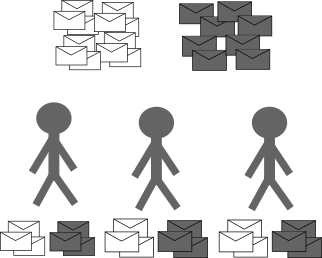
\includegraphics[width=5cm]{img/multiprofile}
\end{center}
    Для классификации используются как собственные письма, так и письма от других пользователей
\end{figure}
\end{frame}
\begin{frame}{Постановка задачи}
\begin{itemize}
	\item Произвести обзор открытых систем фильтрации спама и выбрать средство для расширения.
    \item Реализовать в рамках выбранного средства алгоритм классификации на базе метода опорных векторов в работе А. Розинкина. 
    \item Разработать модификацию метода, которая позволит классифицировать сообщения по нескольким профилям
	\item Реализовать данную модификацию в рамках выбранного ранее средства
    \item Произвести экспериментальное исследование
\end{itemize}
\end{frame}

\begin{frame}{Метод опорных векторов}
\begin{figure}[h]
\begin{center}
    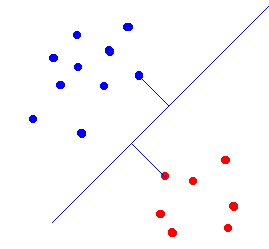
\includegraphics[width=5cm]{../img/svm}
\end{center}
    Разделяющая гиперплоскость максимально удалена от объектов обоих классов
\end{figure}
\end{frame}

\begin{frame}{Представление письма в виде вектора}
\begin{figure}[h]
\begin{center}
    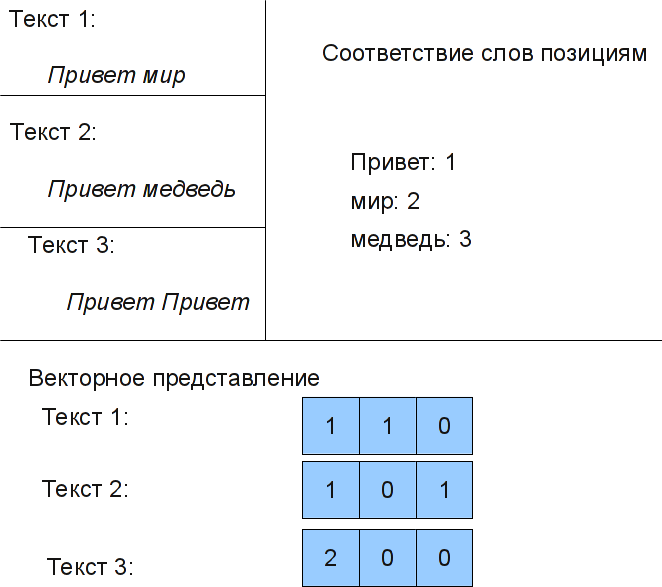
\includegraphics[width=5cm]{../img/vectorize}
\end{center}
    Представление письма в виде вектора
\end{figure}
\end{frame}

\begin{frame}{Многопрофильность}
\begin{figure}[h]
\begin{center}
    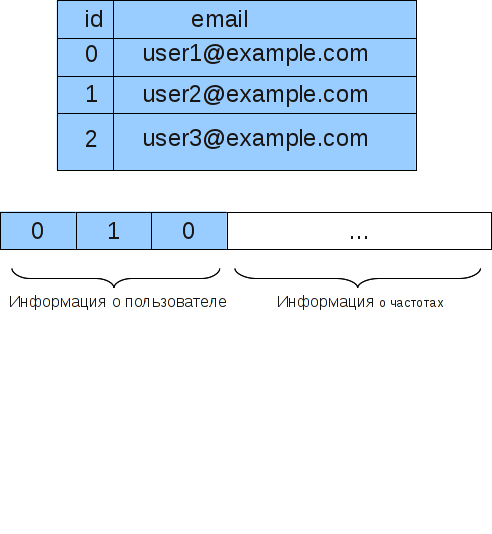
\includegraphics[width=5cm]{../img/add_uid}
\end{center}
	Добавление информации о пользователе
\end{figure}
\end{frame}



\begin{frame}{dspam}
    \begin{itemize}
        \item Свободный
        \item Быстрый
        \item Многопользовательский
    \end{itemize}
\end{frame}

\begin{frame}{Схема работы модифицированного dspam}
\begin{figure}[h]
\begin{center}
    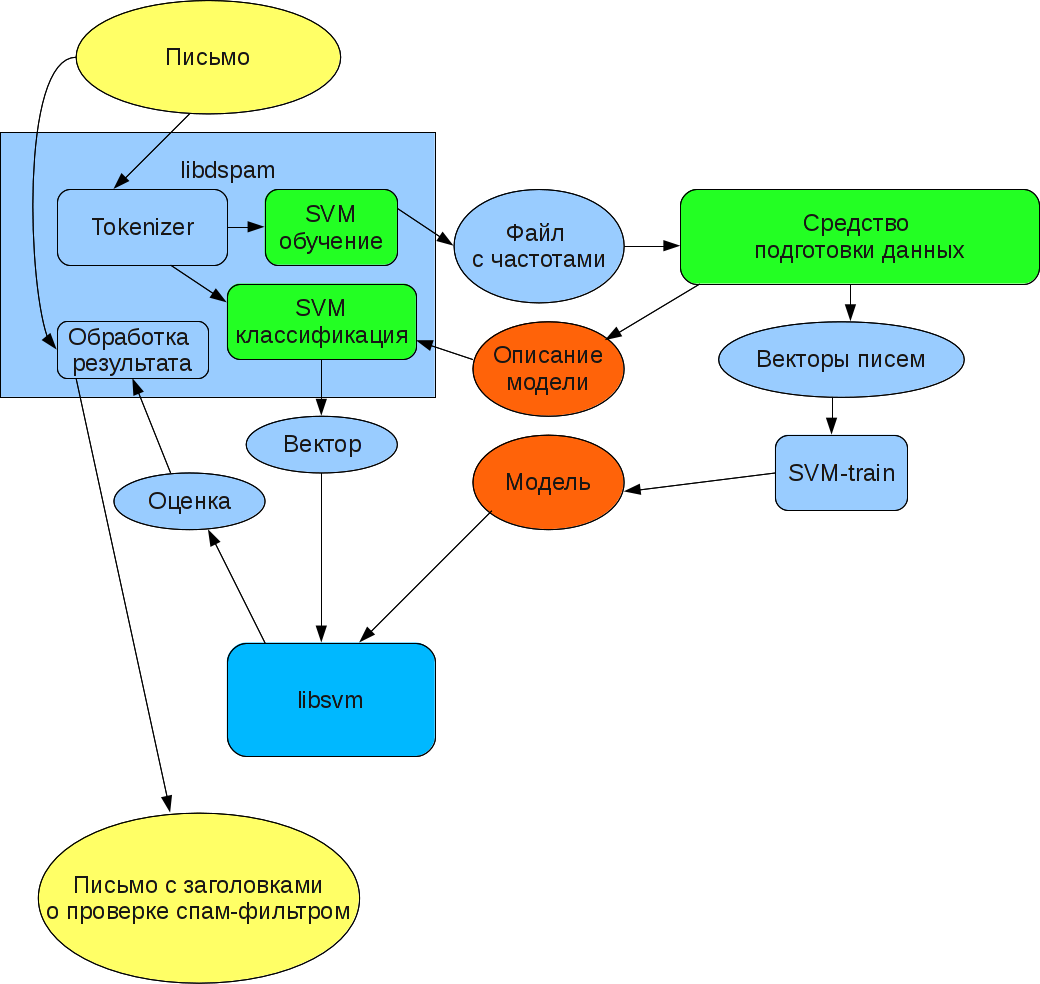
\includegraphics[width=7.5cm]{../img/working_scheme2}
\end{center}
\end{figure}
\end{frame}

\begin{frame}{Результаты тестирования}
\begin{figure}[h]
\begin{center}
    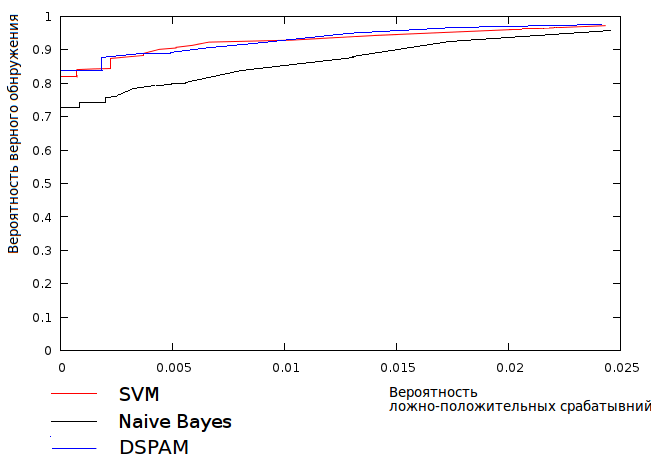
\includegraphics[width=7.5cm]{../img/graphic}
\end{center}
    Соотношение коэффицента верных обнаружений и коэффицента ложных срабатываний
\end{figure}

\end{frame}

%\begin{frame}{Тестирование многопрофильного режима}
%\end{frame}

\begin{frame}{Результаты}
\begin{itemize}
\item Произведен обзор существующих средств фильтрации спама, выбрано средство для доработки.
\item В рамках средства реализован алгоритим фильтрации спама на основе метода опорных векторов, описанный в работе Розинкина.
\item Разработана модификация метода опорных вектров для работы с несколькими профилями.
\item Разработанный метод реализован в рамках системы dspam.
\item Произведено экспериментальное исследование.
\end{itemize}
\end{frame}

\end{document}
